%!TEX root = ../template.tex
%%%%%%%%%%%%%%%%%%%%%%%%%%%%%%%%%%%%%%%%%%%%%%%%%%%%%%%%%%%%%%%%%%%%
%% chapter2.tex
%% NOVA thesis document file
%%
%% Chapter with the template manual
%%%%%%%%%%%%%%%%%%%%%%%%%%%%%%%%%%%%%%%%%%%%%%%%%%%%%%%%%%%%%%%%%%%%

\typeout{NT FILE chapter2.tex}%

\chapter{Background}
\label{cha:background}

\glsresetall


\section{Formal Software Verification}
\label{sec:formal_software_verification}

The quest for proving that a program does what we expect it to do is so important in computer science that it became a branch of it called formal software verification. 
There are several approaches~\cite{DBLP:conf/fm/BrainP24} that try to solve this issue, each one with different characteristics, advantages and disadvantages. 
In this section, we will describe the current situation of the theoretical work and tools that constitute the background of this thesis.


\subsection{Hoare Logic} 
\label{sub:hoare_logic}

Hoare logic~\cite{hoare69} is a way of reasoning about the correctness of a program, following well defined axioms and rules.
The main feature of the Hoare logic is the Hoare triple. 
The name comes from the 3 parts that constitute it: the pre-condition (\emph{P}), the program (\emph{S}) and the post-condition (\emph{Q}):
\[ \{P\} \ \textbf{S} \ \{Q\} \]

This means that if a program \emph{S} satisfies a given pre-condition \emph{P}, the state of the program after the execution finishes satisfies the post-condition \emph{Q}.
To simplify a lot, you can look at the triple as a simple logical consequence \emph{P} $\rightarrow$ \emph{Q}.
In the same way as in the logical consequence, if \emph{P} is false, we can not say anything certain about the value of \emph{Q} (after the execution terminates, in the case of the triple).

Let us now look at an example of the usage of the Hoare triple. Consider the following program:
\[ 
\emph{S} \triangleq \textbf{if } \text{grade} \geq 10 \textbf{ then } \text{reward} := 10 \textbf{ else } \text{reward} := 0 
\]

Hoare logic can be used to prove this triple:
\[
\{ \text{grade} \geq 0 \land \text{grade} \leq 20 \} \, \textbf{S} \, \{ (\text{grade} \geq 10 \land \text{reward} = 10) \lor (\text{grade} < 10 \land \text{reward} = 0) \}
\]

This triple describes a situation where if the value of \emph{grade} is "valid" (considering grades from 0 to 20), we can say that the value of \emph{reward} will be either 0 or 10, depending if the value of \emph{grade} was less than 10 / greater or equal to 10, respectively.
It is also important to mention the difference between \emph{partial correctness} and \emph{total correctness}.
If \emph{total correctness} is what you are looking for, you need to guarantee that the execution of the program finishes.
Otherwise, you can only gurantee \emph{partial correctness}.


\subsection{Relational Hoare Logic} 
\label{sub:relational_hoare_logic}

\subsubsection{Evolution from Classical\protect\footnote{\ When we say Classical Hoare Logic, we mean the original Hoare logic developed by Tony Hoare.} Hoare Logic}
\label{sub:relational_hoare_logic_motivation}

Relational Hoare Logic~\cite{naumann2022thirtysevenyearsrelationalhoare, DBLP:conf/popl/Benton04} (RHL) is a way of reasoning about some property of two different programs or two different executions of the same program.
Some of these properties are observational equivalence and 2-properties, being non-interference and continuity two examples of that concept.
While classical HL reasons about the satisfaction of the post-condition if the pre-condition is satisfied, RHL analyzes the relation between two programs in terms of their corresponding evolution from a given pre-condition to a post-condition.
In other words, if programs \emph{P1} and \emph{P2} both respect the pre-condition (let us name it $\Phi$), they will end (if their executions terminate) both respecting the post-condition (let us name it $\Psi$) or none of them will.
This means that one of the programs satisfying $\Psi$ and the other not satisfying it is not valid in RHL.
This idea is known as the Hoare quadruple:
\[ \{\Phi\} \, \emph{P1} \, \sim \, \emph{P2} \, \{\Psi\} \]

So, why was RHL created when we already had classical HL? 
The main reason lies in the fact that the classical version does not have a direct or easy way of specifying the relation between two programs. 
This would clearly be an obstacle to this work since we aim to prove the correctness of programs by establishing a relation between them and their already proven or versions that are easier to prove.
However, this work is definitely not the only one that relies on the connection between two different implementations of the same of code.
The most common examples are probably compiler optimizations.
Nonetheless, there is another example: when a given program has different algorithms that perform the same task and they get chosen depending on some characteristics that make one implementation more performant than some other(s).


\subsubsection{Detailing RHL with examples}
\label{sub:relational_hoare_logic_examples}

Next, there are some requirements not specified above when presenting the Hoare quadruple.
These are important details that have to be accounted for and will be described using example programs to make the explanation more tangible.
Consider the notation \emph{Pi.j} that will be used in this subsubsection, where \emph{i} represents a given program index, \emph{Pi} refers to a given program and \emph{Pi.j} the identifier of a variable \emph{j} in program \emph{Pi}.

The first example corresponds to two different programs, let us call them \emph{P1} and \emph{P2}, and they both contain only two assignment statements applied to the same group of variables (\emph{a, b, c}): 
\begin{tabbing}
  \hspace{2cm}\= \emph{P1} \hspace{2cm} \= \emph{P2} \\ 
  \> \emph{b := a + 1;} \> \emph{c := a + 2;} \\
  \> \emph{c := b + 1;} \> \emph{b := c - 1;}
\end{tabbing}

We can see that \emph{b} and \emph{c} do not change the final state of any of the programs, so, to write a Hoare quadruple that creates an equivalence between \emph{P1} and \emph{P2}, we need the pre-condition to assert that \emph{P1.a = P2.a}:
\[ \{ \Phi \} \, \emph{P1} \, \sim \, \emph{P2} \, \{ \Psi \} \]
\vspace{-20pt}
\[ where \ \ \Phi \triangleq \text{P1.a} = \text{P2.a} \]
\vspace{-25pt}
\[ and \ \ \Psi \triangleq \text{P1.a} = \text{P2.a} \land \text{P1.b} = \text{P2.b} \land \text{P1.c} = \text{P2.c} \]

This Hoare quadruple should be read as: \emph{If an execution of P1 and P2 guarantee the equality of their x-components, they both diverge from the post-condition or they both finish in states where their x-components, y-components and z-components have the same values
\protect\footnote{\ The values of the components of any of the programs can differ between themselves (\emph{P1.x} has no relation to \emph{P1.y}, for example).}.}

We now introduce the concept of separability.
If two programs \emph{P1} and \emph{P2} utilize disjoint sets of variables, we say that they are \emph{separable}.
Also, in those cases we do not need to specify the program that a given variable belongs to when describing the pre and post conditions.
Below is another example to show the impact on conciseness that this creates.
Consider two programs, \emph{P1}, whose variables are \{{a, b, i, j}\} and \emph{P2} whose variables are \{{a', b', i', j'}\}, meaning that they are separable:
\begin{tabbing}
  \hspace{3cm}\= \emph{P1} \hspace{3cm} \= \emph{P2} \\ 
  \> \emph{a := 1;} \> \emph{a' := 1;} \\
  \> \emph{while a < b do} \> \emph{i' := j' * j';} \\
  \> \emph{\ \ \ \ i := j * j;} \> \emph{while a' < b' do} \\
  \> \emph{\ \ \ \ a := a * i;} \> \emph{\ \ \ \ a' := a' * i';} \\
  \> \emph{od} \> \emph{od} 
\end{tabbing}

What these programs calculate is not the focus here but notice a subtle, yet relevant difference: \emph{i' := j' * j';} is out of the loop in \emph{P2}.
This is a common compiler optimization called \emph{invariant hoisting}.
\emph{Why would you waste time performing a task several times if you can do it only once and get the same output?}
In this example, the Hoare quadruple would be:
\[ \{ \Phi \} \, \emph{P1} \, \emph{\textasciitilde} \, \emph{P2} \, \{ \Psi \} \]
\vspace{-20pt} 
\[ \text{where} \ \ \Phi \triangleq (b = b') \land (j = j') \]
\vspace{-25pt} 
\[ \text{and} \ \ \Psi \triangleq (a = a') \land (b = b') \land (i = i') \land (j = j') \]

Since the previous values in \emph{a} and \emph{i} (respectively \emph{a'} and \emph{i'}) are discarded by the assignments made to these variables, they will have no effect on the final state, so they do not appear in the pre-condition.
On the other hand, to make sure that the components of \emph{P1} and \emph{P2} hold the same values after the executions terminate, we must assert that the n-components and y-components are equal in the initial state of the programs. 

Furthermore, there is a special case of the usage of the Hoare quadruple that does not challenge any concept described before.
Usually, in the context of the Hoare quadruple, we consider that the programs \emph{P1} and \emph{P2} are different, but what would happen if they are exactly the same?
Well, since they are equal letter for letter, it is natural that they will always output the same results given the same inputs.

Finally, consider again two equal programs \emph{P1} and \emph{P2}.
The way one should look at the transformation of Hoare triples into Hoare quadruples is that if \{$\Phi$\} \emph{P1} \emph{\textasciitilde} \emph{P2} \{$\Psi$\} is true, then \{$\phi$\} \emph{P1} \{$\psi$\} will be true as well.


\subsubsection{Axioms and Inference Rules}
\label{sub:relational_hoare_logic_formal_proof_rules}

Consider, for the rules in this subsubsection, that the two given programs \emph{C1} and \emph{C2} are separable.
To derive valid Hoare quadruples, there are axioms and inference rules that reason about the relation between two programs.
We can divide these rules in at least three sets that increment the former set with some additional rules, meaning there is the simplest set, the base set and the extended set.
The simplest set has limitations that we will discuss after presenting them, but is the best starting point:

\begin{figure}[h]
  \centering
  \begin{mathpar}
  \inferrule*[right=skip]
  { }
  {\vdash \{ \Phi \} \ \textbf{skip} \sim \textbf{skip} \ \{ \Phi \}}
  
  \inferrule*[right=assignment]
  { }
  {\vdash \{ \Psi[x_1 \mapsto E_1][x_2 \mapsto E_2] \}  \ x_1 := E_1 \sim x_2 := E_2 \ \{ \Psi \}}
  
  \inferrule*[right=sequencing]
  {\vdash \{ \Phi \} \ C_1 \sim C_2 \ \{ \Theta \} \\\vdash \{ \Theta \} \ C'_1 \sim C'_2 \ \{ \Psi \}}
  {\vdash \{ \Phi \} \ C_1; C'_1 \sim C_2; C'_2 \ \{ \Psi \}}
  
  \inferrule*[right=conditional]
  {\shortstack{%
    $\vDash \Phi \rightarrow (B_1 = B_2)$ \\[0.5ex]%
    $\vdash \{ \Phi \land B_1 \} \ C_1 \sim C_2 \ \{ \Psi \}$ \\%
    $\vdash \{ \Phi \land \neg B_1 \} \ C'_1 \sim C'_2 \ \{ \Psi \}$%
  }}
  {\vdash \{ \Phi \} \ \textbf{if } B_1 \textbf{ then } C_1 \textbf{ else } C'_1 \ \textbf{fi} 
  \sim \textbf{if } B_2 \textbf{ then } C_2 \textbf{ else } C'_2 \ \textbf{fi} \ \{ \Psi \}}

  \inferrule*[right=while]
  {\vdash \{ \Phi \land B_1 \} \ C_1 \sim C_2 \ \{ \Phi \} \\\vDash \Phi \rightarrow (B_1 = B_2)}
  {\vdash \{ \Phi \} \ \textbf{while } B_1 \ \textbf{do } C_1 \ \textbf{od} \sim 
  \textbf{while } B_2 \ \textbf{do } C_2 \ \textbf{od} \ \{ \Phi \}}
  
  \inferrule*[right=weakening]
  {\vDash \Phi' \rightarrow \Phi \\\vdash \{ \Phi \} \ C_1 \sim C_2 \ \{ \Psi \} \\\vDash \Psi \rightarrow \Psi'}
  {\vdash \{ \Phi' \} \ C_1 \sim C_2 \ \{ \Psi' \}}

  \end{mathpar}
  \caption{Simplest set of rules of RHL.}
\end{figure}
  
This set of rules has some considerable limitations however: both programs \emph{C1} and \emph{C2} must be structurally equivalent and execute in lockstep.
This creates a situation where we can not derive a simple Hoare quadruple like \{$\Phi$\} \emph{C}; \textbf{skip} \emph{\textasciitilde} \emph{C} \{$\Psi$\}.
To allow this and other important derivations, we present next other 4 rules that enable the separate reasoning of \emph{C1} and \emph{C2}.
Together with the rules of the simplest set, these rules constitute the base set:

\begin{figure}[h]
  \centering
  \begin{mathpar}

  \inferrule*[right=assignment-L]
    {\vdash \{ \Phi[x \mapsto E] \} \; \textbf{skip} \sim C \; \{ \Psi \}}
    {\vdash \{ \Phi \} \; x := E \sim C \; \{ \Psi \}}

  \inferrule*[right=assignment-R]
    {\vdash \{ \Phi[x \mapsto E] \} \; C \sim \textbf{skip} \; \{ \Psi \}}
    {\vdash \{ \Phi \} \; C \sim x := E \; \{ \Psi \}}

  \inferrule*[right=conditional-L]
    {\vdash \{ \Phi \land B \} \; C_1 \sim C \; \{ \Psi \} \\ 
    \vdash \{ \Phi \land \neg B \} \; C_2 \sim C \; \{ \Psi \}}
    {\vdash \{ \Phi \} \; \textbf{if} \; B \; \textbf{then} \; C_1 \; \textbf{else} \; C_2 \; \textbf{fi} \sim C \; \{ \Psi \}}

  \inferrule*[right=conditional-R]
    {\vdash \{ \Phi \land B \} \; C \sim C_1 \; \{ \Psi \} \\ 
    \vdash \{ \Phi \land \neg B \} \; C \sim C_2 \; \{ \Psi \}}
    {\vdash \{ \Phi \} \; C \sim \textbf{if} \; B \; \textbf{then} \; C_1 \; \textbf{else} \; C_2 \; \textbf{fi} \; \{ \Psi \}}
    
  \end{mathpar}
  \caption{Base set of rules of RHL.}
\end{figure}

Finally, the extended set contains one more rule than the base set: self-composition.
We will not dive deep here on the need of this rule, instead we do it in \hyperref[sec:self_composition]{3.2}.

\begin{figure}[h]
  \centering
  \begin{mathpar}

  \inferrule*[right=self-composition]
    {\vdash \{ \Phi \} \; C_1 ; C_2 \; \{ \Psi \}}
    {\vdash \{ \Phi \} \; C_1 \sim C_2 \; \{ \Psi \}}
    
  \end{mathpar}
  \caption{Extended set of rules of RHL.}
\end{figure}

Note that the premise of this rule is not a Hoare quadruple, but a Hoare triple since there is no \emph{\textasciitilde} operator, only a sequenciation of \emph{C1} and \emph{C2} in a single program.
This triple can also be presented as the following quadruple:
\vspace{-4pt} 
\[ \{\Phi \land \Phi'\} \, \emph{C1 ; C2} \, \sim \, \emph{C1' ; C2'} \, \{ \Psi \land \Psi' \} \]
\vspace{-18pt} 

If we keep the programs \emph{C1;C2} and \emph{C1';C2'} \emph{separable} by renaming their variables and if \emph{$\Phi$ = $\Phi$'} and \emph{$\Psi$ = $\Psi$'}, we get to the self-composition rule in the figure above.


\section{OCaml}
\label{sec:ocaml}

\subsection{History \& Characteristics} 
\label{sub:overview}

OCaml is a general purpose programming language that was released in 1996 at the National Institute for Research in Digital Science and Technology (Inria).
It is usually seen as an extension of Caml (a dialect of the Meta Language) that includes object-oriented features, making OCaml a very versatile language.
Besides supporting the functional, imperative and object-oriented approaches, it is also a language that can be either interpreted or compiled, to either bytecode or native code. 
Regarding its type system, OCaml is strongly and statically typed, featuring type inference as well.

Although the imperative programming paradigm is still more popular than its functional counterpart, the latter has been conquering space inside the universe of programming languages whose focus is on the imperative/object-oriented approach; for example, Java and Kotlin.
%Java received its first functional features in version 1.8, released in 2014 and they have been expanding since.
%Kotlin, on the other hand, was already designed with the functional style in mind,

INSERIR REFERENCIAS!

\subsection{Relevance} 
\label{sub:relevance}

The relevance of OCaml and functional programming languages in general is an important question that I've asked myself several times in the past, and not only because the first contact with this paradigm was challenging.
Although I do not question the relevance of these languages anymore because of the evidence that I will show next, I still think that it is not an unexpected concern among computer science students.
I say this because the majority of jobs and companies in this field require people for front-end development (with Javascript), back-end development (mostly with imperative languages) or, more recently, AI-related work (mostly with Python or other science-oriented languages).
There is, although, strong evidence that OCaml is far from being an "academia only" programming language.
OCaml is used in tech giants such as Meta and Microsoft, in Bloomberg L.P. (that even created an OCaml to Javascript compiler backend) in tools like Docker and in many other companies and businesses.
But wait, there is more! Here are a few impressive examples of what this programming language has been used to build: INSERT LIST HERE
Alt-Ergo, a popular SMT solver that has presence in Cameleer;
Coq, a formal proof management system;
and even the web version of Facebook Messenger!

\subsection{Code Examples} 
\label{sub:examples_ocaml}

In this subsection, we will look at a simple Ocaml code example that determines the greatest common divisor of two given numbers, \emph{a} and \emph{b}.
The first implementation represents the use of the functional paradigm while the second demonstrates how to use imperative constructs in this language.

\begin{ocamlsmall}
  let rec gcd (a: int) (b:int) : int =
      if b = 0 then a
      else gcd b (mod a b) 
\end{ocamlsmall}

\begin{ocamlsmall}
  let gcd_iter (a0: int) (b0: int) : int =
      let b = ref b0 in
      let a = ref a0 in
      while !b <> 0 do
          let tmp = !a in
          a := !b;
          b := tmp mod !b
      done;
      !a
\end{ocamlsmall}

Next there are some notes about the syntax and semantics in the context of the examples above. 
Since OCaml supports the functional and imperative paradigms, it distinguises between immutable variables (actually no presence in the programs above) and memory references, therefore the different syntax for the binding of each one: 
--- INTRODUZIR CENTRADO let x = 3 (variable)
--- INTRODUZIR CENTRADO let y = ref 4 (reference)

The \emph{rec} keyword tells the compiler/interpreter that it is fine if the function calls itself, reducing the risk of the programmer using recursion by accident.
OCaml is also sharp enough to understand these programs correctly even if we did not specify the types of the function or its arguments.
Finally, the \emph{let} keyword can be used to define a function or create a binding, something rather uncommon for someone with an imperative background.


\section{Why3}
\label{sec:why3}

Why3 is a platform whose objective is the verification of programs in a deductive way, presenting it self as a INTRODUZIR CITACAO \emph{"a front-end to third-party theorem provers"}.
These several theorem provers can be put to work together and vary greatly in nature, ranging from SMT solvers (for example, Z3 or cvc5) to TPTP provers and even interactive proof assistants (such as Coq or Isabelle).
Under the hood, Why3 is an OCaml library, implemented in the form of an API.
It features a CLI INTRODUZIR GLOSSARIO, a GUI INTRODUZIR GLOSSARIO and a benchmark tool to compare the performance of the different provers available.


\section{GOSPEL}
\label{sec:gospel}

GOSPEL (Generic Ocaml SPEcification Language) INTRODUZIR REF DO PAPER DE GOSPEL is a tool-agnostic specification language for OCaml that allows one to verify the correctness of a program (there are other purposes but this is the most interesting for this work).
GOSPEL is based in Separation Logic but significantly improves the experience of the people that write and/or read the specifications, by making them much more concise.
%Se acessibilty and conciseness aspects, which are considered by its authors "two downsides that, we believe, limit its wide adoption" INSERIR CITACAO!.
Let us reconsider the code presented in the subsection above, but this time also show the GOSPEL specification for that program:

\begin{gospel}
  (*@ function rec gcd (a: int) (b:int) : int =
      if b = 0 then a
      else gcd b (mod a b) *)
  (*@ requires a >= 0
      requires b >= 0
      variant b *)
\end{gospel}

\begin{gospel}
  let gcd_iter (a0: int) (b0: int) : int =
    let b = ref b0 in
    let a = ref a0 in
    while !b <> 0 do
        (*@ invariant 0 <= !b
            invariant 0 <= !a
            invariant gcd a0 b0 = gcd !a !b
            variant !b *)
        let tmp = !a in
        a := !b;
        b := tmp mod !b
    done;
    !a
  (*@ result = gcd_iter a0 b0
      requires a0 >= 0
      requires b0 >= 0
      ensures result = gcd a0 b0*)
\end{gospel}

Although this a simple program, we can already notice what a typical GOSPEL specification looks like.
If we are dealing with a functional piece of code usually there will be a few \emph{requires} clauses (could be none as well) at the beginning of the specification, representing the pre-conditions.
After that, since these implementations use recursion most of the time, there will be one or more \emph{variant} clauses, indicating what variables vary each the function is called.
This serves as a guarantee that the recursion does not go forever.
In this implementation, \emph{variant b} is enough but we could eventually reason about how \emph{a} varies over the execution of the program. 
Regarding the pre-conditions, this particular example states that \emph{a} and \emph{b} need to be non negative integer numbers, since the greatest common divisor of any two negative numbers will always be 0.
Finally, we have a single post-condition \emph{ensures result = gcd a0 b0} that guarantees that for any input, the two different implementations will output the same result. 


\section{Cameleer}
\label{sec:cameleer}

Cameleer is a tool that aids automated deductive verification of OCaml programs.
It relies on GOSPEL for the specification of the code and on Why3 to effectively verify the program.
The limitations of the powerful Why3 tool and the reason for the creation of Cameleer start here: Why3 does not accept code that is not written in its intermediary language: WhyML.
Now imagine wanting to verify your codebase with years and years of contributions, with maybe more than a million lines of code.
Why3 would force you to translate OCaml into WhyML, \emph{all by hand}. 
And only after that you would write the specification.
Two obvious things come to mind: no one wants to do that job and if someone had to do it, they would very quickly start wondering if there is a tool that could help them, or even better, do that repetitive work instead of them.
So, how is Cameleer able to save those poor programmers?

\begin{figure}[htbp]
  \centering
  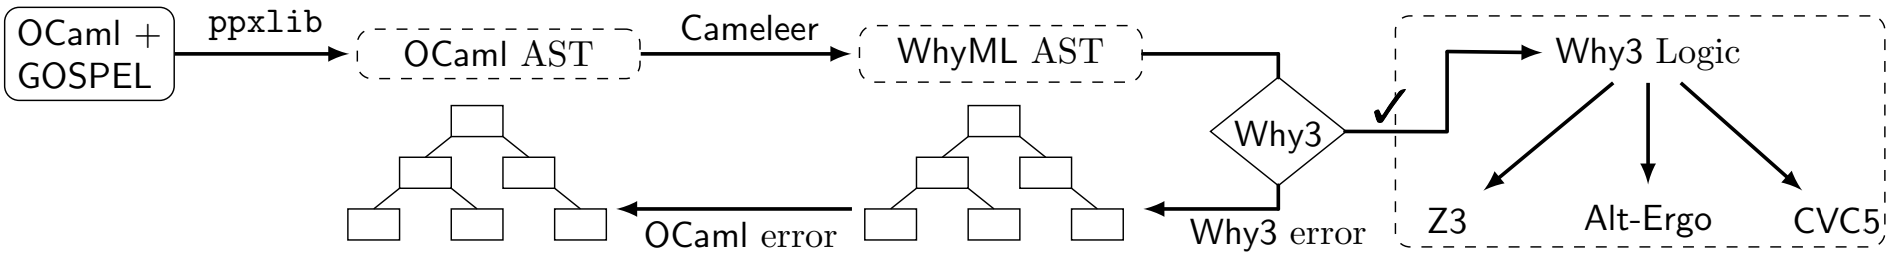
\includegraphics{cameleer_pipeline}
  \caption{Architecture and verification pipeline, taken from INTRODUZIR REFERENCIA.}
  \label{fig:cameleer_pipeline}
\end{figure}

The Cameleer pipeline is constituted by 4 different steps, the last one being different depending on whether Why3 detects errors in the translated code or not.
The first step is to parse and change the abstract syntax tree of the input OCaml program (that contains GOSPEL annotations), using \emph{ppxlib}, a library that is part of the GOSPEL ecosystem INSERIR FOOTNOTE GITHUB DE GOSPEL.
In the second step, the GOSPEL annotations are processed by a special parser/type-checker that converts the specification into nodes that become part of the previous OCaml AST.
The third step consists in Cameleer itself translating the complete AST into a description in WhyML that is equivalent; Why3 then takes that as input.
In step four, if the Why3 type-and-effect system is not able to validate the input generated in the previous step, the problems are shown in the context of the input OCaml code, the one that is submitted by the user. 
Alternatively, if no errors are found, a series of verification conditions are the output of the respective VCGEN.
Those VCs should then be unraveled by the solvers featured in Cameleer or, if they are not able to do all the work automatically, this tool also allows human intervention to discharge more complex statements.

